% This file was created by matlab2tikz.
%
%The latest updates can be retrieved from
%  http://www.mathworks.com/matlabcentral/fileexchange/22022-matlab2tikz-matlab2tikz
%where you can also make suggestions and rate matlab2tikz.
%
\documentclass[tikz]{standalone}
\usepackage[T1]{fontenc}
\usepackage[utf8]{inputenc}
\usepackage{pgfplots}
\usepackage{grffile}
\pgfplotsset{compat=newest}
\usetikzlibrary{plotmarks}
\usetikzlibrary{arrows.meta}
\usepgfplotslibrary{patchplots}
\usepackage{amsmath}
\let\inf\relax \DeclareMathOperator*\inf{\vphantom{p}inf}
\begin{document}
\definecolor{mycolor1}{rgb}{0.00000,0.44700,0.74100}%
\definecolor{mycolor2}{rgb}{0.85000,0.32500,0.09800}%
%
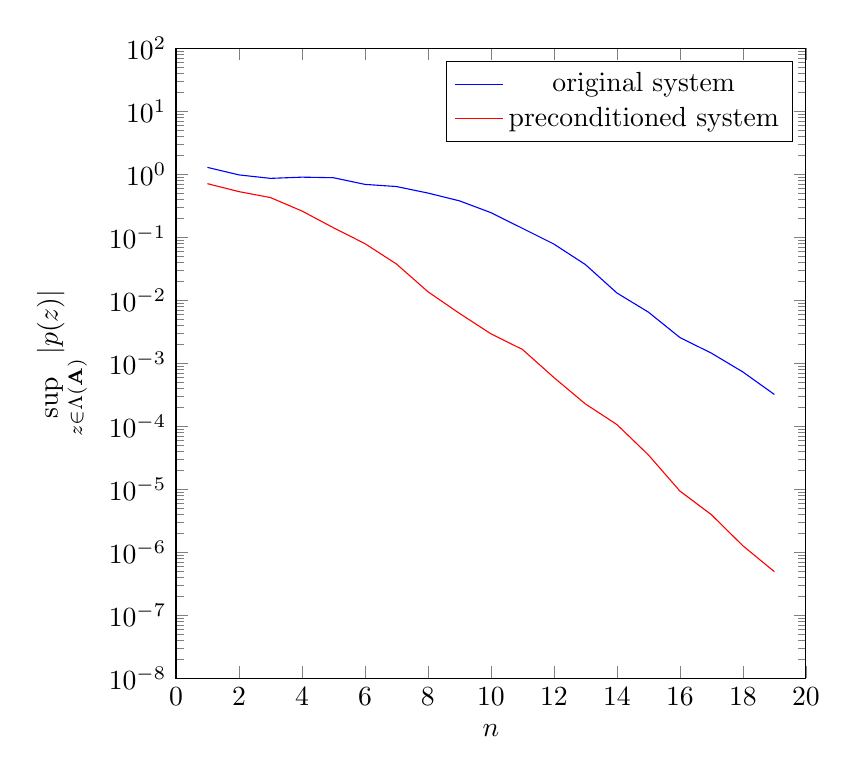
\begin{tikzpicture}

\begin{axis}[%
width=8cm,
height=8cm,
at={(0cm,0cm)},
scale only axis,
xmin=0,
xmax=20,
ymode=log,
ymin=1e-08,
ymax=100,
xlabel={$n$},
ylabel={$\sup\limits_{z\in \Lambda(\mathbf{A})} |p(z)|$},
yminorticks=true,
axis background/.style={fill=white}
]
\addplot [color=blue]
  table[row sep=crcr]{%
1	1.28\\
2	0.973\\
3	0.857\\
4	0.896\\
5	0.878\\
6	0.688\\
7	0.636\\
8	0.501\\
9	0.377\\
10	0.245\\
11	0.138\\
12	0.0776\\
13	0.0367\\
14	0.013\\
15	0.00645\\
16	0.00255\\
17	0.00144\\
18	0.000724\\
19	0.000318\\
};
\addplot [color=red]
  table[row sep=crcr]{%
1	0.706\\
2	0.528\\
3	0.425\\
4	0.26\\
5	0.141\\
6	0.0789\\
7	0.0375\\
8	0.0136\\
9	0.00617\\
10	0.00292\\
11	0.00165\\
12	0.000591\\
13	0.000225\\
14	0.000106\\
15	3.49e-05\\
16	9.32e-06\\
17	3.93e-06\\
18	1.26e-06\\
19	4.89e-07\\
};
\legend{original system, preconditioned system};
\end{axis}
\end{tikzpicture}%
\end{document}